\documentclass[12pt]{extarticle}
\usepackage[utf8]{inputenc}
\usepackage[english]{babel}

% \usepackage[disable]{todonotes}
% \usepackage{todonotes}
% \newcommand{\dg}[1]{\todo[inline]{DG: #1}}
\usepackage{siunitx}
\usepackage{graphicx}
\usepackage{xcolor}
\usepackage{wrapfig}
\usepackage[compact]{titlesec}

% Pollock
\definecolor{C0}{HTML}{000000}
\definecolor{C1}{HTML}{511818}
% \definecolor{C2}{HTML}{3b4666}
\definecolor{C2}{HTML}{1c4bab}
\definecolor{C3}{HTML}{222ee0}
\definecolor{C4}{HTML}{a04540}

\usepackage[%
% hidelinks,
% bookmarksopen=true,
% colorlinks=true,
% citebordercolor={1 0 0},
% citecolor=red,
% urlbordercolor={0 0 1},
pdfborderstyle={/S/U/W 1},
% linkbordercolor=C2,
% urlbordercolor=C2,
% urlcolor=C2%
urlbordercolor=C2,
urlcolor=C3%
]{hyperref}
% \urlstyle{same}
\usepackage[inline]{enumitem}
\usepackage[a4paper, top=2.2cm, bottom=2.2cm, left=2.4cm, right=2.4cm]{geometry}
\usepackage{microtype}

% A font combination which does not scream LaTeX
\usepackage{tgpagella}
\usepackage{eulervm}

\usepackage{setspace}

\newif\iftwocolloc
\twocolloctrue
% \twocollocfalse
\iftwocolloc\usepackage{multicol}\else{}\fi

\newcommand*\sq{\mathbin{\vcenter{\hbox{\rule{.8ex}{.8ex}}}}}
\newcommand*\ssq{\mathbin{\vcenter{\hbox{\rule{.6ex}{.6ex}}}}}
\newenvironment{t_sq_itemize}
{\begin{itemize}[topsep=0pt, parsep=0pt, itemsep=0pt, leftmargin=*]
    \renewcommand{\labelitemi}{{\(\sq\)}}}
  {\end{itemize}}

\begin{document}
\color{C0}


\noindent
To: Natasha Timofeyuk \newline
Chair of the European Research Committee \newline
on Few-Body Problems in Physics

\bigskip
\noindent
\doublespacing
  \noindent
  {\Large Conference proposal:}

  \bigskip
\doublespacing
\noindent{\color{C2}\fontfamily{qag}\selectfont%
  \LARGE\bf  26th  European Conference on
  Few-Body Problems in Physics (EFB26)} \newline
{\Large Prague, Czech Republic, July--August 2026}\\
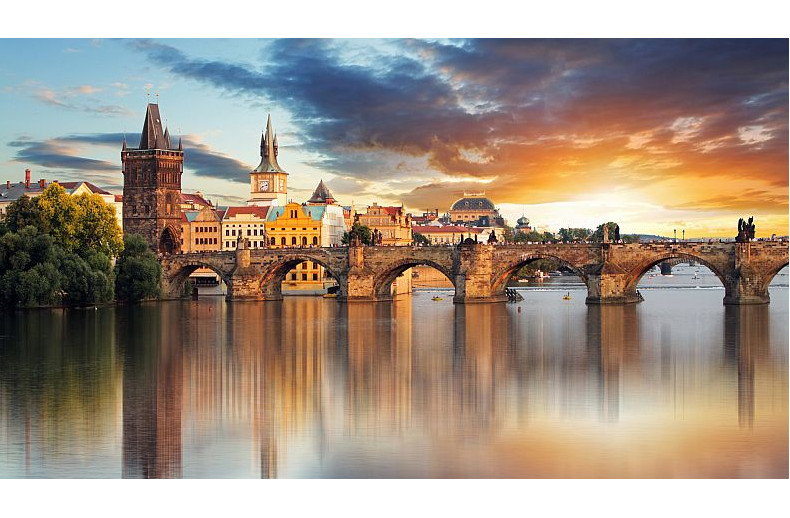
\includegraphics[width=1.0\textwidth]{Prague_foto_cut}

\onehalfspacing
\section*{Venue and Host Institutions}
\noindent
The EFB26 conference will take place in Prague in 2026, one week in
the period July--August. It will be hosted by the
\href{http://www.ujf.cas.cz/en/}{Nuclear Physics Institute} (ÚJF)
of the
\href{https://www.avcr.cz/en/}{Czech Academy of Sciences} (CAS);
\href{https://www.mff.cuni.cz/en}{Faculty of Mathematics and
  Physics} (MFF), \href{https://cuni.cz/UKEN-1.html}{Charles
  University} (CUNI);
and
\href{https://www.jh-inst.cas.cz/}{The Heyrovský Institute of Physical
  Chemistry} (JH), CAS.

\paragraph{Charles University} (Latin: Universitas Carolina) is the
largest university in the Czech Republic, ranked amongst the top
\qty{2}{\percent} of universities in the world. Being founded in 1348,
it is one of the oldest universities in Europe in continuous
operation. Faculty of Mathematics and Physics, CUNI carries out
research and training in physics, mathematics and computer science.

\paragraph{The Czech Academy of Sciences} is the leading
non-university research institution in the Czech Republic. Its
tradition goes back to the Royal Bohemian Society of Sciences founded
in 1784. The Academy conducts research in a broad spectrum of natural,
technical, and social sciences and humanities. The Nuclear Physics
Institute, CAS conducts research in nuclear physics, experimental as
well as theoretical. The Heyrovský Institute of Physical Chemistry,
CAS promotes the scientific legacy of the Nobel laureate,
Jaroslav Heyrovský, in fields related to physical chemistry.

\paragraph{Prague} with its rich history and stunning architecture is
one of the world's most popular tourist destinations. Prague was
ranked the 6th in the Tripadvisor world list of best destinations in
2016 (the 5th in 2014), and it was ranked the 7th in the world ICCA
Destination Performance Index measuring performance of conference
tourism in 2021.

\paragraph{Conference venue} The LOC is currently considering two
options for the conference site:
\begin{t_sq_itemize}
\item
  Faculty of Mathematics and Physics, Charles University
  (\href{https://maps.app.goo.gl/YLm43Nb5XHHziMX16}{Troja Campus})
  -- less expensive but farther from the city center
  \item Congress center ``\href{https://www.masarykovakolej.cz/en/im-organizing-event}{Masarykova Kolej}'' -- more expensive but better
    accessible, Prague Castle is in walking distance
  \end{t_sq_itemize}
  \begin{center}
    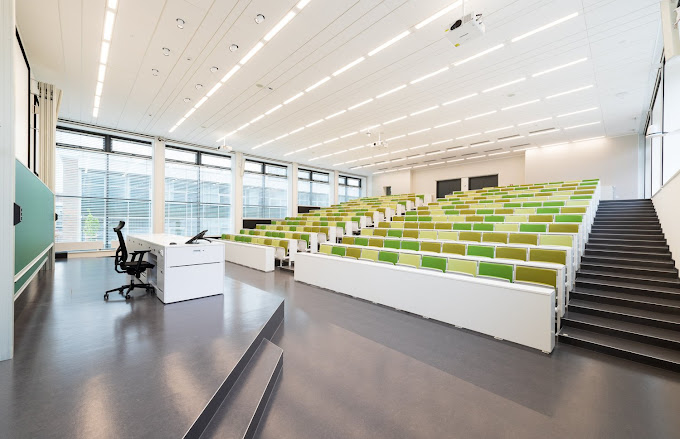
\includegraphics[height=5cm]{Impakt-troja_1}
    \hspace{7mm}
    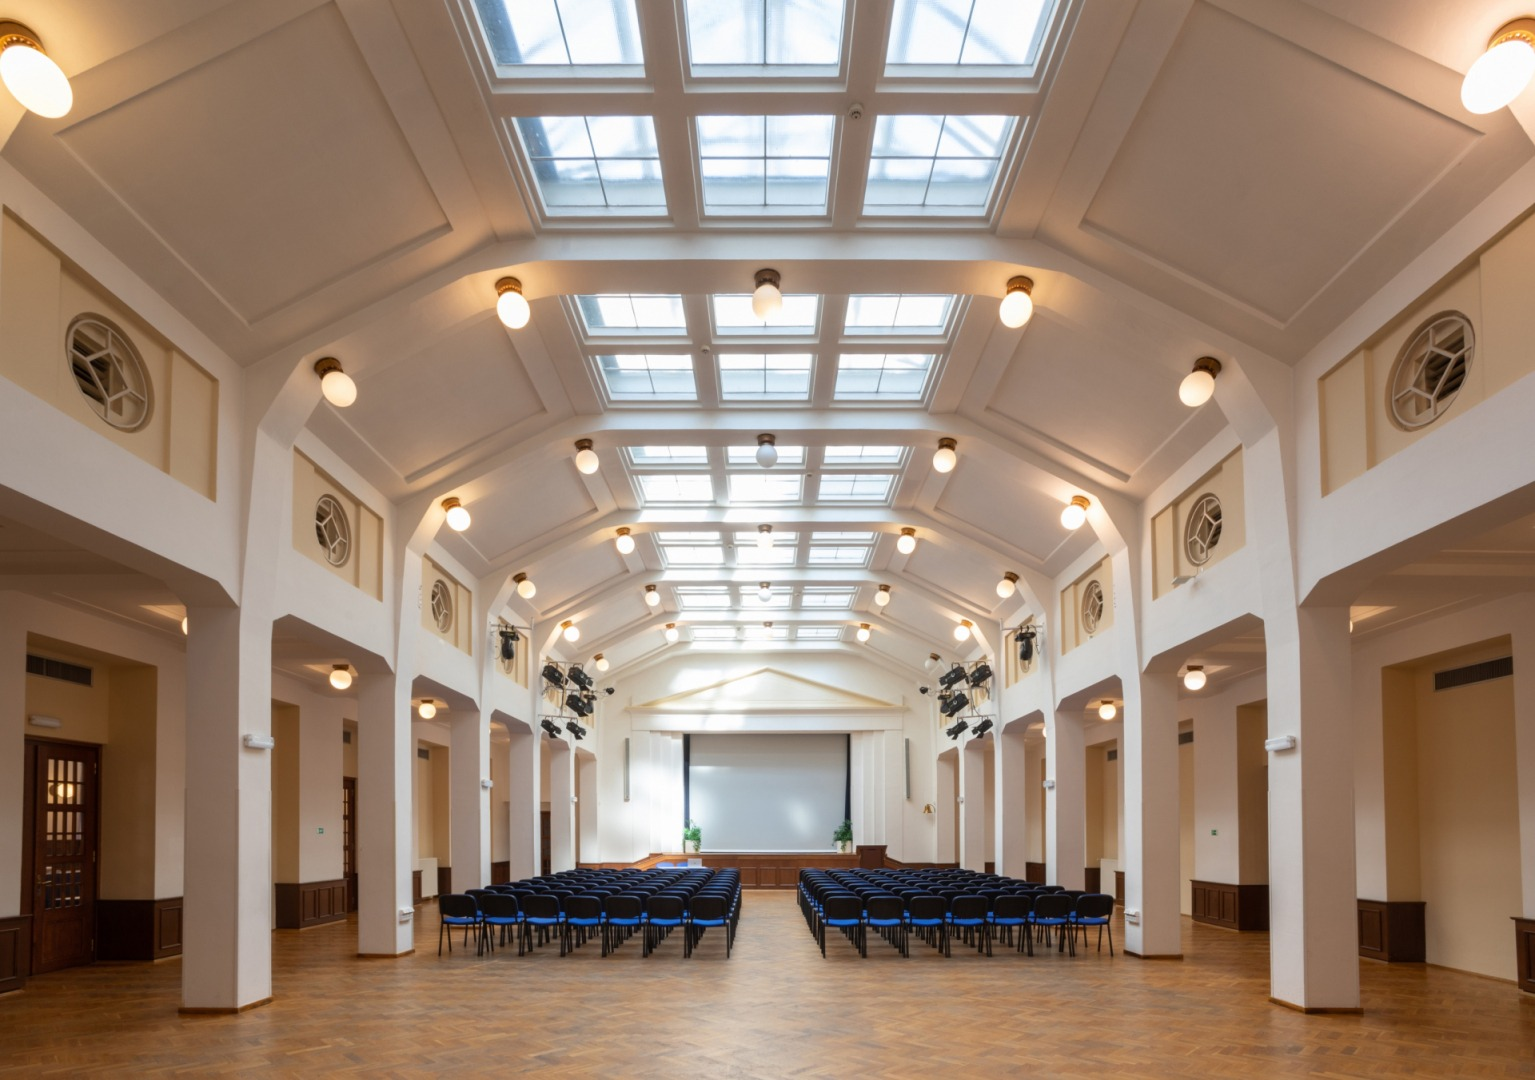
\includegraphics[height=5cm]{MK}\\[-1.5mm]
    \hspace{3mm}{\small Troja Campus}\hspace{5.4cm}{\small Masarykova Kolej}
  \end{center}

\section*{Travel}
\noindent
Due to its location in the heart of Europe, Prague is easily
accessible by plane, train, bus or car. Prague has an extensive public
transport network that is rated as one of the best and most reliable
in Europe.
% {\bf Troja Campus, transport:} It is possible to travel to Troja by public transport, the closest bus stops being “Kuchyňka”
% and “Pelc Tyrolka”. Alternatively, the campus is about 15 minutes walk from the metro station “Nádraží Holešovice”
% (line C). It is also possible to drive to the campus by car. It is possible to park in front of the main entrance or in the courtyard;
% parking is free and accessible nonstop.


\section*{Local Organizing Committee}
\noindent
The conference will be organized by scientists exploring few-body
phenomena in diverse fields of physics and chemistry. The local
organizing committee will include:
\iftwocolloc\begin{multicols}{2}\else{}\fi
\begin{t_sq_itemize}
  \def\ujf{ÚJF}%{ÚJF AVČR, Řež}
  \def\jh{JH}%{JH AVČR, Prague}
  \def\mff{MFF}%{MFF UK, Prague}
\item Nina Shevchenko, chair (\ujf)
\item Martin Čížek (\mff)
\item Zdeněk Doležal (\mff)
\item Tomáš Dytrych (\ujf)
\item Juraj Fedor (\jh)
\item[]{}
\item Daniel Gazda (\ujf)
\item Karel Houfek (\mff)
\item Jiří Mareš (\ujf)
\item Zdeněk Mašín (\mff)
\end{t_sq_itemize}
\iftwocolloc\end{multicols}\else{}\fi

\iftwocolloc\noindent\else{}\fi
The members of LOC have ample experience with organizing various
scientific conferences, workshops and schools, such as: ICHEP (2020,
2024), HYP 2022, IMAMPC 2022, AttoChem Prague 2022, Mesons \& Light
Nuclei (1998, 2001), 2nd Conf.\ Cost Action MultiChem 2023, EMMI
Workshop Trieste 2023, DEA workshop 2018, several ECT* workshops in
Trento, more than 30 years of Indian-Summer School of Physics.

\section*{International Advisory Committee and time schedule}
\noindent
The members of IAC will be selected from the lists of advisors from
past EFB conferences. New members could be added after consultation
with the European Few-Body Research Committee to ensure that all areas
of few-body research are covered.

The IAC will be established in summer 2024, when the members will be
asked to suggest invited speakers. The first announcement of the EFB26
conference will be done in autumn 2024, the web page should be already
available at that time.

\section*{Topics}
\noindent
The following topics will be covered at the conference:
\begin{t_sq_itemize}
\item Nuclei and hypernuclei
\item Hadron physics
\item Electroweak processes
\item Nuclear astrophysics
\item Cold atoms and quantum gases
\item Atoms and molecules
\item Few-body methods
\item Few-body aspects of many-body systems
\end{t_sq_itemize}

\section*{Scientific program}
\noindent
The conference will maintain the traditional structure of few-body
conferences lasting 5 days, from Monday to Friday. We will leave
Wednesday afternoon for excursions and/or discussions. There will be
plenary sessions in the mornings and parallel sessions in the
afternoons. There will be about 30 plenary talks lasting 30 minutes
each, including the talks of the Young Researcher Award winners.
Depending on the total number of participants, there will be either
two or three parallel sessions. There will be a poster session as
well. We also plan to host a public lecture of general interest for
participants and the public on a topic related to the conference
theme.

\section*{Proceedings}
\noindent
At the moment, we plan to publish the EFB26 proceedings online or to
adopt the scheme of the EFB25 conference, namely to publish oral
contributions and selected posters in a special issue of the journal
Few-Body Systems if possible. We intend to discuss this issue with the
members of IAC since the proceedings costs could increase the fee by
\(\approx 50\)~EUR.

\section*{Social program}
\noindent
Social program will include a welcome reception, conference dinner,
Prague city center sightseeing and excursions to experimental
laboratories.

\section*{Budget, registration fee}
\noindent
We assume 150 participants, including 30 students, in estimating the
conference fee. We also took into account promised financial
contribution from ÚJF. We intend to apply for a NUPECC support. Of
course, we will make efforts to find other sponsors in order to reduce
the fee and support young participants in particular.

\paragraph{The registration fee} will include conference kit, coffee
breaks, lunches, welcome reception, conference dinner, excursions, and
possibly proceedings. It will be also used to cover the costs of the
conference center including audio-visual equipment, and the costs of
the public lecture. Lunches will be arranged directly at the
conference site or in walking distance.

We will have an early-bird registration fee and reduced fee for
students. No on-line participants are planned. The fee for
accompanying persons will include welcome reception, conference
dinner, public lecture, and excursions. We intend to keep the fees at
the level of the EFB25 conference:
\begin{table}[h]
  \centering
  \begin{tabular}{ll}
    \hline \\[-1mm]
    &   Price in EUR  \\[1mm]
    \hline \\[-1mm]
    Early-bird fee & 500  \\[1mm]
    Full fee &  550 \\[1mm]
    % Early-bird student fee & 350  \\[1mm]
    % Full student fee &  400 \\[1mm]
    Student fee &  350 \\[1mm]
    Accompanying person fee & 100  \\[1mm]
    \hline
  \end{tabular}
\end{table}


%Fee for an accompanying person will include welcome reception and the conference dinner (?).
%{\bf Plus:} 
%We show our estimates in the Table below which includes both lower and higher estimates. The upper
%estimate is calculated assuming a conservative possible rise of 20 \% in prices in three years time.  
%CZK/EUR exchange rate (CZK = Czech koruna) will also play a role (1 EUR = 24.66 CZK at 25.10.23).
%

\section*{Accommodation}
\noindent
Accommodation will not be included in the registration fee and must be
organized by the participants. Prague offers many possibilities for
accommodation which can be found using usual booking portals.

We intend to arrange accommodation for the EFB26 participants at
reduced rates in selected hotels during the time of the conference.
The typical current costs per night in 3/4* hotels are about
75--110~EUR.

\paragraph{For students} we plan to arrange inexpensive accommodation
at nearby dormitories.

\section*{Other information}

\paragraph{Academic and Medical Conference Agency (AMCA)}
Services of AMCA will be used for registration, collection of the
conference fee, editing and printing of the book of abstract,
catering, social dinner.

\paragraph{Visa requirements}
Czech Republic does not require visas from EU/EEA citizens for stays
of any duration or for any purpose. Citizens of
\href{https://www.mzv.cz/jnp/en/information_for_aliens/short_stay_visa/list_of_states_whose_citizens_are_exempt/index.html}{several
  non-Schengen countries} do not need a visa for non-profit stays of
up to 90 days. However, citizens of some
\href{https://www.mzv.cz/jnp/en/information_for_aliens/short_stay_visa/list_of_states_whose_citizens_are/index.html}{other
  countries} might require a visa to enter the Czech Republic (see
\texttt{www.mzv.cz}).

% We will provide
% letters of invitation to those participants who need visas well in
% advance and will recommend they apply for the visa well in advance.

\paragraph{Weather}
The Czech Republic has a temperate climate, situated in the transition
zone between the oceanic and continental climate types, with warm
summers. July and August are the warmest months of the year. On
average, summer day temperatures are about
\qty[parse-numbers=false]{20-30}{\celsius}
(\qty[parse-numbers=false]{70-90}{\degree F}). Occasional showers and
thunderstorms can be expected.
\end{document}


%%%%%%%%%%%%%%%%%%%%%%%%%%%%%%%%%%%%%%%%
For one-column wide figures use syntax of figure~\ref{fig-1}
%\begin{figure}[h]
% Use the relevant command for your figure-insertion program
% to insert the figure file.
%\centering
%\includegraphics[width=1cm,clip]{tiger}
%\caption{Please write your figure caption here}
%\label{fig-1}       % Give a unique label
%\end{figure}

For figure with sidecaption legend use syntax of figure
%\begin{figure}
% Use the relevant command for your figure-insertion program
% to insert the figure file.
%\centering
%\sidecaption
%\includegraphics[width=5cm,clip]{tiger}
%\caption{Please write your figure caption here}
%\label{fig-3}       % Give a unique label
%\end{figure}
